\documentclass[a4paper,12pt]{article}

\usepackage{amsfonts, amsmath, amssymb, amsthm, enumitem, fancyhdr, graphicx}
\usepackage[margin=1in, includehead, includefoot, heightrounded]{geometry}
\allowdisplaybreaks
\pagestyle{fancy}
\rhead{Erick Lin}

\newcommand{\norm}[1]{\left\lVert#1\right\rVert}
\renewcommand{\thesubsection}{\arabic{subsection}}
\newtheorem{theorem}{Theorem}
\newtheorem{lemma}[theorem]{Lemma}

\begin{document}

\section*{MATH 4640 -- HW3 Solutions}
\begin{enumerate}
    \item
        Suppose $i, j \in [0, \cdots, k]$ are arbitrary. $l_i(x) = 0$ for all $x$ where $x \neq x_i$, and likewise $l_j(x) = 0$ for all $x$ where $x \neq x_j$, so $l_i(x) l_j(x) = 0$ for all $x \in \{ x_0, \cdots, x_k \}$. Also, both $l_i(x)$ and $l_j(x)$ are products of $k$ terms, so $l_i(x) l_j(x)$ is of degree $2k$. Since $x_0, \cdots, x_k$ are the $k + 1$ zeros of $p_{k + 1}(x)$ and $\deg(p_{k + 1}(x)) < \deg(l_i(x) l_j(x))$, $p_{k + 1}(x)$ must divide $l_i(x) l_j(x)$. Thus, $l_i(x) l_j(x) = p_{k + 1}(x) g(x)$ where $\deg(g(x)) = k - 1 \leq k$, so $g(x)$ can be written in the basis $p_0, p_1, \cdots, p_k$, from which we can deduce that $p_{k + 1} g(x) = 0$. In conclusion, $l_i(x) l_j(x)$; i.e., $l_i(x)$ and $l_j(x)$ are orthogonal.
    \item
        \iffalse
            Since $\sin \pi x$ is $2$-periodic, we first give an approximation for $\sin x$ which is $2\pi$-periodic. We know that the trigonometric polynomial $f_2(x)$ of degree $\leq 2$ that minimizes
            \begin{align*}
                %\norm{\sin x - f_2(x)}_{L^2} =
                \int_0^{2\pi} (\sin x - f_2(x))^2 dx
            \end{align*}
            is given by
            \begin{align*}
                f_2(x) &= \sum_{k = -2}^2 c_k e^{ikx}, \qquad c_k = \langle \sin x, e^{ikx} \rangle = \frac{1}{2\pi} \int_0^{2\pi} \sin x e^{-ikx} dx \\
                &= \frac{1}{2\pi} \left[ 0 + i\pi(e^{-ix}) + 0 - i\pi(e^{ix}) + 0 \right] \\
                &= \frac{i(e^{-ix} - e^{ix})}{2} = \sin x
                %\left( \frac{e^{-2\pi ik} - 1}{k^2 - 1} \right) e^{-ikx}
            \end{align*}
        \fi
        Take the first three terms of the sequence of Legendre polynomials $p_0(x) = 1$, $p_1(x) = x$, $p_2(x) = \frac{1}{2}(3x^2 - 1)$ which are orthogonal under the inner product $\langle f(x), g(x) \rangle = \int_{-1}^1 f(x)g(x)dx$. Then the least squares (sub)quadratic approximation to $\sin \pi x$ on $[-1, 1]$ is given by
        \begin{align*}
            p(x) &= \sum_{i = 0}^2 \frac{\langle \sin \pi x, p_i(x) \rangle}{\langle p_i(x), p_i(x) \rangle} p_i(x) \\
            &= 0 + \frac{\int_{-1}^1 x \sin\pi x dx}{\int_{-1}^1 x^2 dx}x + 0 \\
            &= \frac{-\frac{x\cos\pi x}{\pi}|_{-1}^1 - \int_{-1}^1 \frac{\cos \pi x}{\pi} dx}{\frac{x^3}{3}|_{-1}^1} x \\
            &= \frac{\frac{2}{\pi} - \frac{1}{\pi} \sin\pi x|_{-1}^1}{\frac{2}{3}} x \\
            &= \frac{3}{\pi} x \\
            &\approx 0.95493x.
        \end{align*}

    \item
        Since $f(x) = f(x + 2\pi)$ for all $x$ by assumption, we have that $g_\alpha(x) = f(x - \alpha) = f(x - \alpha + 2\pi) = g_\alpha(x + 2\pi)$ for all $x$. \par
        Thus, $\hat{f}(j) = \hat{g}_\alpha(j)$ because
        \begin{align*}
            \hat{g}_\alpha(j) &= \frac{1}{2\pi} \int_0^{2\pi} f(x - \alpha) e^{-ijx} dx \\
            &= \frac{e^{-ij\alpha}}{2\pi} \int_\alpha^{2\pi + \alpha} f(y) e^{-ijy} dy \text{ (using the change of variable $y = x + \alpha$)} \\
            &= \frac{e^{-ij\alpha}}{2\pi} \left( \int_\alpha^{2\pi} + \int_{2\pi}^{2\pi+\alpha} \right) f(y) e^{-ijy} dy \\
            &= \frac{e^{-ij\alpha}}{2\pi} \left( \int_\alpha^{2\pi} + \int_0^{\alpha} \right) f(y) e^{-ijy} dy \\
            &= \frac{e^{-ij\alpha}}{2\pi} \int_0^{2\pi} f(y) e^{-ijy} dy = e^{-ij\alpha} \hat{f}(j).
        \end{align*}

    \item
        $f(x)$ is continuous because each piece is continuous as a polynomial function and at $x = \pi$, $(\pi/\pi)^2 - \pi/\pi = 0 = (\pi - \pi)/\pi - ((\pi - \pi)/\pi)^2$. Also, the first piece at $x = 0$ agrees with the last piece at $x = 2\pi$ since $(0/\pi)^2 - 0/\pi = 0 = (2\pi - \pi)/\pi - ((2\pi - \pi)/\pi)^2$. \par
        Likewise,
        \begin{align*}
            f'(x) = \begin{cases}
                2x/\pi^2 - 1/\pi, &0 \leq x < \pi \\
                1/\pi - 2(x - \pi)/\pi^2, &\pi \leq x < 2\pi
            \end{cases}
        \end{align*}
        is continuous because each piece remains a polynomial function after differentiation and at $x = \pi$, $2\pi/\pi^2 - 1/\pi = 1/\pi = 1/\pi - 2(\pi - \pi)/\pi^2$; the first piece at $x = 0$ agrees with the last piece at $x = 2\pi$ as $2(0)/\pi^2 - 1/\pi = -1/\pi = 1/\pi - 2(2\pi - \pi)/\pi^2$.
        However, the pieces in
        \begin{align*}
            f''(x) = \begin{cases}
                2/\pi^2, &0 \leq x < \pi \\
                -2/\pi^2, &\pi \leq x < 2\pi
            \end{cases}
        \end{align*}
        agree nowhere. \par
        The spectrum of $f(x)$ is
        \begin{align*}
            \hat{f}(j) &= \frac{1}{2\pi} \int_0^{2\pi} f(x) e^{-ijx} dx \\
            &= \frac{1}{2\pi} \left( \int_0^{\pi} \left[ \left( \frac{x}{\pi} \right)^2 - \frac{x}{\pi} \right] e^{-ijx} dx + \int_\pi^{2\pi} \left[ \frac{x - \pi}{\pi} - \left( \frac{x - \pi}{\pi} \right)^2 \right] e^{-ijx} dx \right) \\
            &= \frac{1}{2\pi} \left[ \left( \frac{1}{\pi j^2} + \frac{e^{-ij\pi}}{\pi j^2} + \frac{2i}{\pi^2 j^3} - \frac{2i e^{-ij\pi}}{\pi^2 j^3} \right) + \left( -\frac{e^{-2ij\pi}}{\pi j^2} - \frac{e^{-ij\pi}}{\pi j^2} + \frac{2ie^{-2ij\pi}}{\pi^2 j^3} - \frac{2i e^{-ij\pi}}{\pi^2 j^3} \right) \right] \\
            &= \frac{1}{2\pi^2 j^2} \left( 1 - e^{-2ij\pi} + -\frac{2i(1 - 2e^{-ij\pi} + e^{-2ij\pi})}{\pi j} \right) \\
            &= -\frac{4i(1 - e^{-ij\pi})}{2\pi^3 j^3},
        \end{align*}
        and so $\hat{f}(j) = O(1/j^3)$.

    \item
        The functions for parts (a) and (b) are respectively plotted below. In the case where $f(x) = \sin^2(3x)$, while we can see that $g_5(x) = 0.5$ for all $x$, it is interesting to note that $g_6(x) = 0.5 - 0.5\cos 6x$ turns out to be $f(x)$ exactly due to a trigonometric power identity. \par
        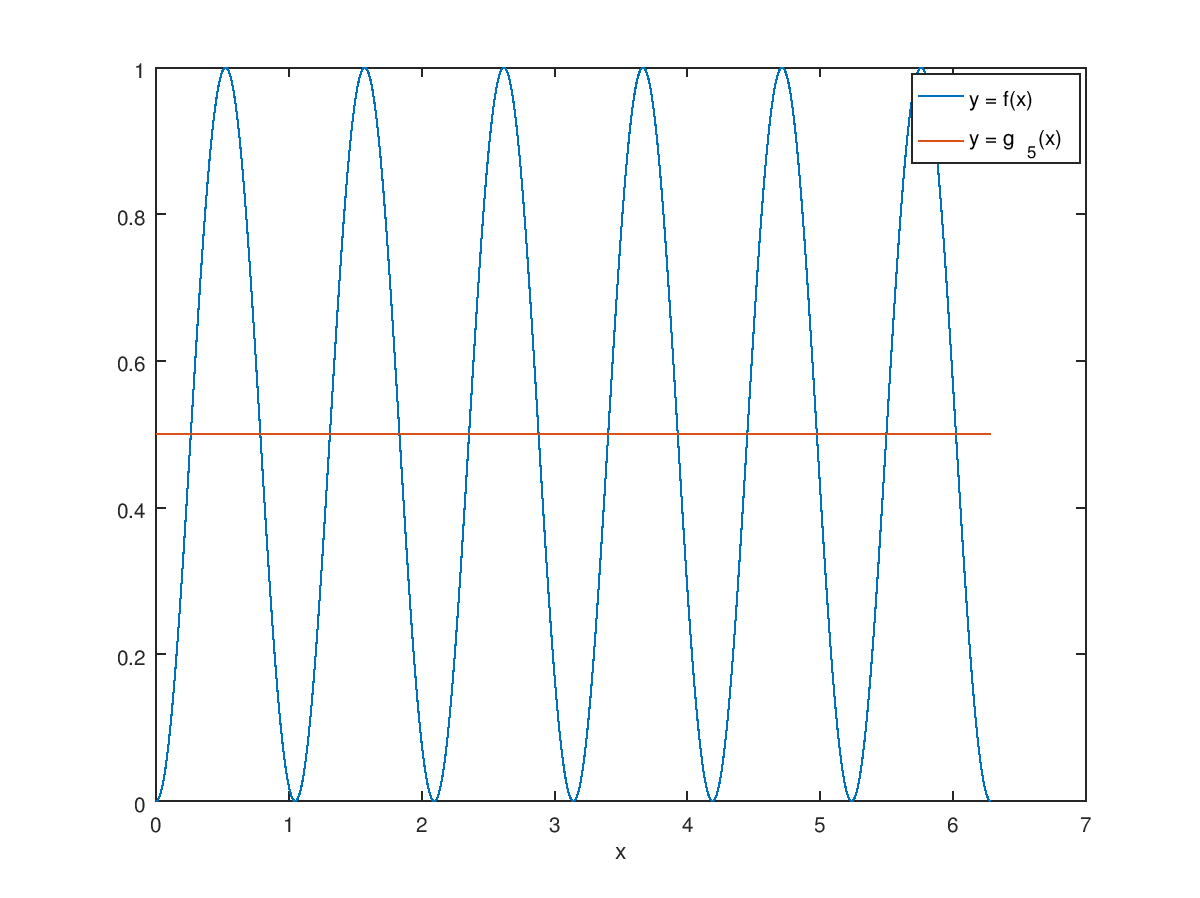
\includegraphics[scale=0.25]{hw3_5a}
        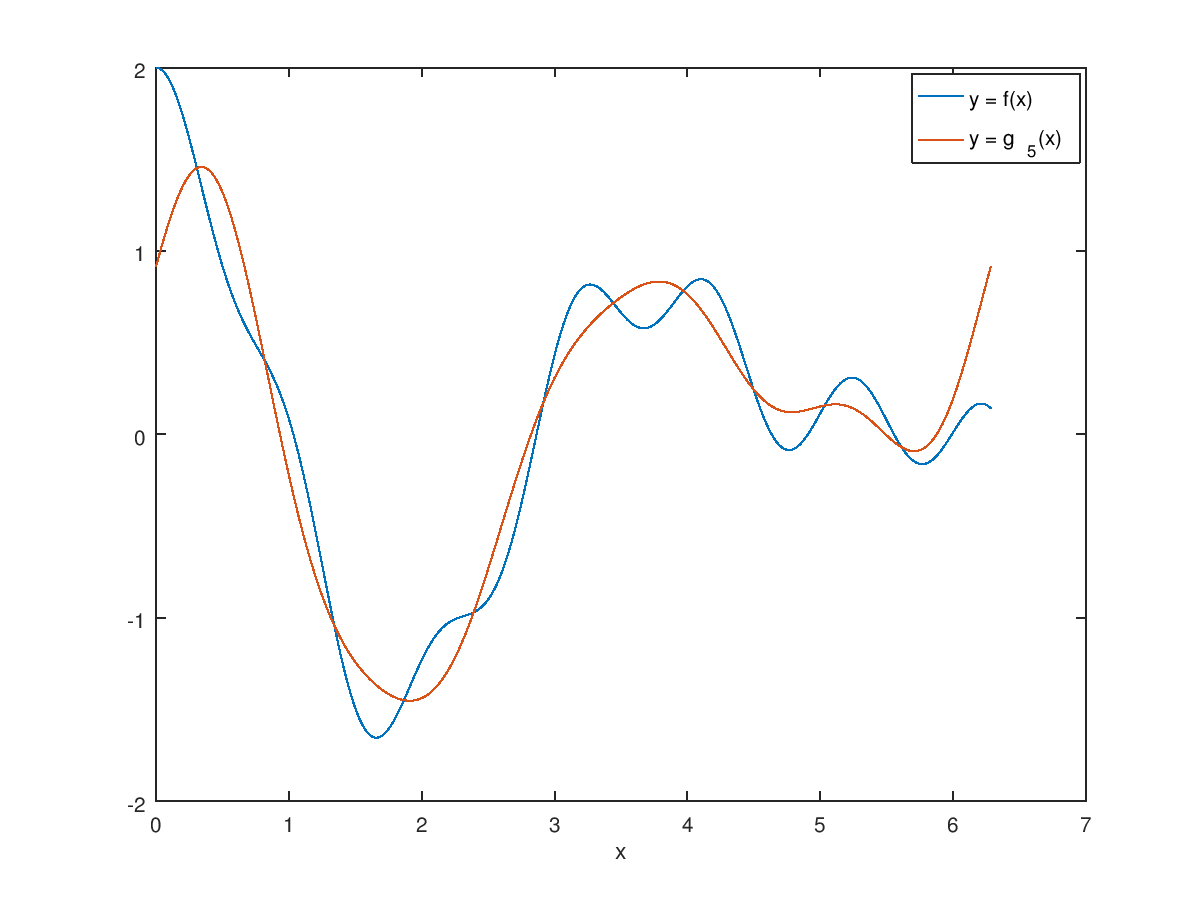
\includegraphics[scale=0.25]{hw3_5b}

    \item
        The Taylor expansions of the polynomials are
        \begin{align*}
            f(a + h) = \sum_{k = 0}^\infty \frac{f^{(k)}(a) \cdot h^k}{k!} \quad \text{and} \quad f(a - h) = \sum_{k = 0}^\infty \frac{f^{(k)}(a) \cdot (-h)^k}{k!},
        \end{align*}
        and thus
        \begin{align*}
            \frac{f(a + h) - f(a - h)}{2h} = \sum_{k = 0}^\infty \frac{f^{(2i + 1)}(a) \cdot h^{2i}}{(2i + 1)!}.
        \end{align*}
        The error is given by
        \begin{align*}
            \left| \frac{f(a + h) - f(a - h)}{2h} - f'(a) \right| = \left| \sum_{k = 1}^\infty \frac{f^{(2i + 1)}(a) \cdot h^{2i}}{(2i + 1)!} \right|.
        \end{align*}

    \item
        By the product rule, differentiating gives
        \begin{align*}
            f'(x) &= p'_k(x) + f[x_0, \cdots, x_k, x] \phi'_k(x) + f[x_0, \cdots, x_k, x, x] \phi_k(x) \\
            f''(x) &= p''_k(x) + f[x_0, \cdots, x_k, x] \phi''_k(x) + 2f[x_0, \cdots, x_k, x, x] \phi'_k(x) \\
            &\quad+ f[x_0, \cdots, x_k, x, x, x] \phi_k(x) \\
            f'''(x) &= p'''_k(x) + f[x_0, \cdots, x_k, x] \phi'''_k(x) + 3f[x_0, \cdots, x_k, x, x] \phi''_k(x) \\
            &\quad+ 3f[x_0, \cdots, x_k, x, x, x] \phi'_k(x) + f[x_0, \cdots, x, x, x, x] \phi_k(x)
        \end{align*}
        and so
        \begin{align*}
            f'''(a) &= p'''_k(a) + f[x_0, \cdots, x_k, a] \phi'''_k(a) + 3f[x_0, \cdots, x_k, a, a] \phi''_k(a) \\
            &\quad+ 3f[x_0, \cdots, x_k, a, a, a] \phi'_k(a) + f[x_0, \cdots, a, a, a, a] \phi_k(a).
        \end{align*}
        Assuming the given conditions, we have
        \begin{align*}
            \phi_3(x) &= (x - a)(x - (a - h))(x - (a + h))(x - (a + 2h)) \\
            &\Rightarrow \phi_3(a) = 0 \\
            \phi'_3(x) &= (x - a)(x - (a - h))(x - (a + h)) + (x - a)(x - (a - h))(x - (a + 2h)) \\
            &\quad+ (x - a)(x - (a + h))(x - (a + 2h)) \\
            &\quad+ (x - (a - h))(x - (a + h))(x - (a + 2h)) \\
            &\Rightarrow \phi'_3(a) = h(-h)(-2h) = 2h^3 \\
            \phi''_3(x) &= 2(x - a)(x - (a - h)) + 2(x - a)(x - (a + h)) \\
            &\quad+ 2(x - (a - h))(x - (a + h)) + 2(x - a)(x - (a + 2h)) \\
            &\quad+ 2(x - (a - h))(x - (a + 2h)) + 2(x - (a + h))(x - (a + 2h)) \\
            &\Rightarrow \phi''_3(a) = 2h(-h) + 2h(-2h) + 2(-h)(-2h) = -2h^2 \\
            \phi'''_3(x) &= 6(x - a) + 6(x - (a - h)) + 6(x - (a + h)) + 6(x - (a + 2h)) \\
            &\Rightarrow \phi'''_3(a) = 6h + 6(-h) + 6(-2h) = -12h.
        \end{align*}
        The error term is given by
        \begin{align*}
            &|f'''(a) - p'''_k(a)| = \bigl| {-12}f[a - h, a, a + h, a + 2h, a]h \\
            &\qquad{} - 6f[a - h, a, a + h, a + 2h, a, a]h^2 + 6f[a - h, a, a + h, a + 2h, a, a, a]h^3 \bigr| \\
            &\quad{} \leq \max_{\xi \in [a - h, a + 2h]} \left[ 12 \left( \frac{f^{(4)}(\xi)}{4!} \right)h + 6 \left( \frac{f^{(5)}(\xi)}{5!} \right)h^2 + 6 \left( \frac{f^{(6)}(\xi)}{6!} \right)h^3 \right].
        \end{align*}
\end{enumerate}

\end{document}
